% ============================================================
%  يُترجَم بـ XeLaTeX  (في Overleaf: Menu → Compiler → XeLaTeX)
%  الخط: Amiri (متوفر في Overleaf، أو حمّله من github.com/aliftype/amiri)
% ============================================================
\documentclass[12pt,a4paper]{article}
\usepackage[a4paper,margin=1.7cm,top=2.3cm,bottom=2.9cm,headheight=15pt,footskip=1.5cm]{geometry}
\usepackage{amsmath,amssymb}
\usepackage{icomma}
\usepackage[english,bidi=default,layout=lists]{babel}
\babelprovide[import,main]{arabic}
\babelfont{rm}[Scale=1.08]{Amiri}
\babelfont{sf}[Scale=1.08]{Amiri}
\usepackage[most]{tcolorbox}
\usepackage{tikz}
\usetikzlibrary{arrows.meta,calc,shadings}
\usepackage{array}
\usepackage{colortbl}
\usepackage{fancyhdr}
\usepackage{titlesec}
\usepackage{enumitem}
\usepackage{collcell}
\usepackage{needspace}
\usepackage{etoolbox}
\newcolumntype{C}{>{\collectcell\ar}c<{\endcollectcell}}
\pretocmd{\section}{\Needspace{15\baselineskip}}{}{}
\pretocmd{\subsection}{\Needspace{11\baselineskip}}{}{}

\definecolor{cDef}{HTML}{1F4E9C}
\definecolor{cThm}{HTML}{B3261E}
\definecolor{cRem}{HTML}{2E7D32}
\definecolor{cEx}{HTML}{C76B00}
\definecolor{cMeth}{HTML}{6A1B9A}
\definecolor{cSol}{HTML}{00695C}
\definecolor{cSec}{HTML}{1F3A68}

\titleformat{\section}{\Large\bfseries\color{cSec}}{\thesection.}{0.6em}{}[{\color{cSec!60}\titlerule[1pt]}]
\titleformat{\subsection}{\large\bfseries\color{cThm!85!black}}{\thesubsection.}{0.5em}{}
\titlespacing*{\section}{0pt}{14pt}{8pt}
\titlespacing*{\subsection}{0pt}{10pt}{5pt}
\setlength{\parindent}{0pt}
\setlength{\parskip}{4pt}
\setlist{itemsep=2pt,topsep=3pt}

\newtcolorbox{arbox}[3][]{enhanced,
  colback=#2!5,colframe=#2!80!black,arc=2mm,boxrule=0.8pt,
  left=6pt,right=6pt,top=8pt,bottom=5pt,
  fonttitle=\bfseries,coltitle=white,
  title={\foreignlanguage{arabic}{#3}},
  attach boxed title to top right={xshift=-5mm,yshift=-3mm},
  boxed title style={colback=#2!80!black,arc=1.5mm,boxrule=0pt},
  before upper={\selectlanguage{arabic}},
  before skip=8pt,after skip=8pt,breakable,#1}
\newenvironment{BOX}[2]{\begin{otherlanguage}{english}\begin{arbox}{#1}{#2}}{\end{arbox}\end{otherlanguage}}
\newenvironment{tarif}[1][تعريف]{\begin{BOX}{cDef}{#1}}{\end{BOX}}
\newenvironment{khassia}[1][خاصية]{\begin{BOX}{cThm}{#1}}{\end{BOX}}
\newenvironment{molahada}[1][ملاحظة]{\begin{BOX}{cRem}{#1}}{\end{BOX}}
\newenvironment{mithal}[1][مثال]{\begin{BOX}{cEx}{#1}}{\end{BOX}}
\newenvironment{tariqa}[1][طريقة]{\begin{BOX}{cMeth}{#1}}{\end{BOX}}

\newcounter{exo}
\newenvironment{tamrin}[1]{\stepcounter{exo}\begin{BOX}{cSec}{التمرين \theexo: #1}}{\end{BOX}}
\newenvironment{hal}{\Needspace{12\baselineskip}\begin{otherlanguage}{english}\begin{arbox}[breakable]{cSol}{حل التمرين \theexo}}{\end{arbox}\end{otherlanguage}}

\newenvironment{LTR}{\begin{otherlanguage}{english}}{\end{otherlanguage}}
\newcommand{\ar}[1]{\foreignlanguage{arabic}{#1}}

\renewcommand{\dots}{\mathinner{\ldotp\ldotp\ldotp}}
\renewcommand{\ldots}{\mathinner{\ldotp\ldotp\ldotp}}
\renewcommand{\cdots}{\mathinner{\cdotp\cdotp\cdotp}}
\newcommand{\N}{\mathbb{N}}
\newcommand{\Z}{\mathbb{Z}}
\newcommand{\D}{\mathbb{D}}
\newcommand{\Q}{\mathbb{Q}}
\newcommand{\R}{\mathbb{R}}
\newcommand{\pgcd}{\operatorname{PGCD}}
\newcommand{\ppcm}{\operatorname{PPCM}}

% \NLseg{a}{b}{[}{]} ; \NLright{a}{[} ; \NLleft{b}{]}  (interval on a number line)
\newcommand{\NLseg}[4]{\begin{LTR}\begin{tikzpicture}[baseline=-0.6ex]
 \draw[-{Stealth[length=2mm]},gray!70](0,0)--(3.4,0);
 \draw[line width=2pt,cThm!80!black](0.7,0)--(2.7,0);
 \node[cThm!80!black,font=\LARGE] at (0.7,0){$#3$};
 \node[cThm!80!black,font=\LARGE] at (2.7,0){$#4$};
 \node[below=3pt,font=\footnotesize] at (0.7,0){$#1$};
 \node[below=3pt,font=\footnotesize] at (2.7,0){$#2$};
\end{tikzpicture}\end{LTR}}
\newcommand{\NLright}[2]{\begin{LTR}\begin{tikzpicture}[baseline=-0.6ex]
 \draw[-{Stealth[length=2mm]},gray!70](0,0)--(3.4,0);
 \draw[line width=2pt,cThm!80!black](1.3,0)--(3.3,0);
 \node[cThm!80!black,font=\LARGE] at (1.3,0){$#2$};
 \node[below=3pt,font=\footnotesize] at (1.3,0){$#1$};
\end{tikzpicture}\end{LTR}}
\newcommand{\NLleft}[2]{\begin{LTR}\begin{tikzpicture}[baseline=-0.6ex]
 \draw[-{Stealth[length=2mm]},gray!70](0,0)--(3.4,0);
 \draw[line width=2pt,cThm!80!black](0.05,0)--(2.1,0);
 \node[cThm!80!black,font=\LARGE] at (2.1,0){$#2$};
 \node[below=3pt,font=\footnotesize] at (2.1,0){$#1$};
\end{tikzpicture}\end{LTR}}

% ---------- social-media icons (pure TikZ) ----------
\definecolor{cFB}{HTML}{1877F2}
\definecolor{cTG}{HTML}{229ED9}
\definecolor{cIG1}{HTML}{FEDA75}
\definecolor{cIG2}{HTML}{D62976}
\definecolor{cIG3}{HTML}{4F5BD5}
\newcommand{\fbicon}{\begin{LTR}\begin{tikzpicture}[baseline=-0.75ex,x=1em,y=1em]
 \fill[cFB] (0,0) circle (0.55);
 \node[white,inner sep=0,font=\usefont{TU}{lmss}{bx}{n}\small] at (0.04,-0.02) {f};
\end{tikzpicture}\end{LTR}}
\newcommand{\igicon}{\begin{LTR}
\begin{tikzpicture}[baseline=-0.75ex,x=1em,y=1em]
 \shade[lower left=cIG1,lower right=cIG2,upper left=cIG2,upper right=cIG3,rounded corners=0.28em] (-0.55,-0.55) rectangle (0.55,0.55);
 \draw[white,line width=0.09em,rounded corners=0.18em] (-0.36,-0.36) rectangle (0.36,0.36);
 \draw[white,line width=0.09em] (0,0) circle (0.17);
 \fill[white] (0.22,0.22) circle (0.05);
\end{tikzpicture}\end{LTR}}
\newcommand{\tgicon}{\begin{LTR}
\begin{tikzpicture}[baseline=-0.75ex,x=1em,y=1em]
 \fill[cTG] (0,0) circle (0.55);
 \fill[white] (-0.33,0.0) -- (0.32,0.27) -- (0.2,-0.3) -- (0.0,-0.15) -- (-0.08,-0.28) -- (-0.08,-0.08) -- cycle;
 \fill[cTG!70!black] (-0.08,-0.08) -- (0.25,0.2) -- (0.0,-0.15) -- (-0.08,-0.28) -- cycle;
\end{tikzpicture}\end{LTR}}
% page number: black box, white two-digit number, at the right of the social row
\newcommand{\PageBox}{\begin{LTR}\tikz[baseline=(p.base)]\node[fill=black,text=white,inner sep=2.5pt,minimum width=1.6em,minimum height=1.3em,font=\usefont{TU}{lmss}{bx}{n}\small](p){\ifnum\value{page}<10 0\fi\arabic{page}};\end{LTR}}
% visual left-to-right order: Telegram | Instagram | Facebook | page box
\newcommand{\SocialRow}{\begin{otherlanguage}{english}%
 \ar{\textbf{الأستاذ سوايسية هشام للرياضيات}}\ \tgicon\hfill
 \textbf{prof\_hicham\_math}\ \igicon\hfill
 \ar{\textbf{الأستاذ سوايسية هشام للرياضيات}}\ \fbicon\hspace{2.2em}\PageBox\end{otherlanguage}}

\pagestyle{fancy}
\fancyhf{}
\renewcommand{\headrulewidth}{0.6pt}
\renewcommand{\footrulewidth}{0.4pt}
% \SetHeader{right head: document title}{left head: level -- stream}
\newcommand{\SetHeader}[2]{%
 \fancyhead[C]{\parbox{\textwidth}{\ar{#1\hfill #2}}}%
 \fancyfoot[C]{\parbox{\textwidth}{\small\SocialRow}}}
\usepackage{tkz-tab}
\usepackage{multicol}
% variation / sign table (LTR)
\newenvironment{TAB}{\par\begin{center}\begin{LTR}\begin{tikzpicture}[scale=0.95,every node/.style={font=\small}]}{\end{tikzpicture}\end{LTR}\end{center}}
% grid + axes, clipped: \begin{GR}{xmin}{xmax}{ymin}{ymax}{unit cm}
\newenvironment{GR}[5]{\par\begin{center}\begin{LTR}\begin{tikzpicture}[x=#5cm,y=#5cm,font=\footnotesize]
 \draw[gray!25,very thin] (#1,#3) grid (#2,#4);
 \draw[-{Stealth[length=2mm]}] (#1,0)--(#2+0.3,0) node[below left]{$x$};
 \draw[-{Stealth[length=2mm]}] (0,#3)--(0,#4+0.3) node[below left]{$y$};
 \node[below left] at (0,0){$O$};
 \begin{scope}\clip (#1,#3) rectangle (#2,#4);}
{\end{scope}\end{tikzpicture}\end{LTR}\end{center}}
\newcommand{\Ticks}[2]{\foreach \t in {#1} \node[below,font=\scriptsize] at (\t,0){$\t$}; \foreach \t in {#2} \node[left,font=\scriptsize] at (0,\t){$\t$};}
\newcommand{\bx}[1]{\ensuremath{\colorbox{cDef!12}{$\displaystyle #1$}}}
\newcommand{\TwoCol}[4]{\par\begin{LTR}\noindent\begin{minipage}[t]{#1\textwidth}\selectlanguage{arabic}#2\end{minipage}\hfill\begin{minipage}[t]{#3\textwidth}\selectlanguage{arabic}#4\end{minipage}\end{LTR}\par}
\newcommand{\RL}[4]{\TwoCol{#3}{#4}{#1}{#2}}  % \RL{w1}{right content}{w2}{left content}
\newcommand{\ok}{$\textcolor{cRem}{\checkmark}$}
\newcommand{\limn}{\displaystyle\lim_{n\to+\infty}}
% sub-questions, each on its own line
\newenvironment{sq}{\begin{itemize}[leftmargin=2.4em,itemsep=3pt]}{\end{itemize}}
\newcommand{\qa}{\item[(أ)]}\newcommand{\qb}{\item[(ب)]}\newcommand{\qc}{\item[(جـ)]}\newcommand{\qd}{\item[(د)]}\newcommand{\qe}{\item[(هـ)]}
\newcommand{\pa}{\par\smallskip\textbf{(أ)} }\newcommand{\pb}{\par\smallskip\textbf{(ب)} }\newcommand{\pc}{\par\smallskip\textbf{(جـ)} }\newcommand{\pd}{\par\smallskip\textbf{(د)} }\newcommand{\pe}{\par\smallskip\textbf{(هـ)} }
\newcommand{\QQ}[1]{\par\smallskip\textbf{#1.} }
\newenvironment{tmr}{\stepcounter{exo}\begin{BOX}{cSec}{تمرين محلول \theexo}}{\end{BOX}}
\newcommand{\ABC}[3]{\\[2pt]\begin{tabular}{p{0.28\textwidth}p{0.28\textwidth}p{0.28\textwidth}}(جـ) \ #3 & (ب) \ #2 & (أ) \ #1\end{tabular}}
\pretocmd{\section}{\Needspace{24\baselineskip}}{}{}
\newtcbox{\bxtbox}{on line,colback=cDef!12,colframe=cDef!12,boxrule=0pt,arc=1pt,boxsep=0pt,left=2pt,right=2pt,top=1pt,bottom=1pt}
\newcommand{\bxt}[1]{\foreignlanguage{english}{\bxtbox{\ar{#1}}}}
% complex plane: \begin{CP}{xmin}{xmax}{ymin}{ymax}{unit cm}
\newenvironment{CP}[5]{\par\begin{center}\begin{LTR}\begin{tikzpicture}[x=#5cm,y=#5cm,font=\footnotesize]
 \draw[gray!22,very thin] (#1,#3) grid (#2,#4);
 \draw[-{Stealth[length=2mm]}] (#1,0)--(#2+0.4,0);
 \draw[-{Stealth[length=2mm]}] (0,#3)--(0,#4+0.4);
 \draw[thick,-{Stealth[length=2mm]}] (0,0)--(1,0) node[pos=0.55,below]{$\vec u$};
 \draw[thick,-{Stealth[length=2mm]}] (0,0)--(0,1) node[pos=0.55,left]{$\vec v$};
 \node[below left] at (0,0){$O$};}
{\end{tikzpicture}\end{LTR}\end{center}}
\newcommand{\Pt}[3][above right]{\fill (#2) circle (1.7pt) node[#1,inner sep=2pt]{$#3$};}
\SetHeader{\small\bfseries\color{cSec}ملخص: الأعداد المركبة والتحويلات النقطية}{\small\color{cSec}السنة الثالثة ثانوي -- الشعب العلمية}
\let\origNeedspace\Needspace
\renewcommand{\Needspace}[1]{\origNeedspace{14\baselineskip}}
\begin{document}
\begin{LTR}
\begin{tcolorbox}[enhanced,colback=cSec,colframe=cSec,arc=3mm,halign=center,boxrule=0pt,top=12pt,bottom=12pt,before upper={\selectlanguage{arabic}}]
{\color{white}\fontsize{26}{32}\selectfont\bfseries الأعداد المركبة والتحويلات النقطية}\\[8pt]
{\color{white}\large ملخص شامل مع أمثلة وأشكال وتمارين محلولة خطوة بخطوة}\\[5pt]
{\color{white}\large السنة الثالثة ثانوي -- الشعب العلمية}
\end{tcolorbox}
\end{LTR}

\begin{BOX}{cSec}{محتوى الملخص}
\begin{enumerate}[label=\textbf{\arabic*.}]
\item المجموعة $\mathbb{C}$ والشكل الجبري، التمثيل الهندسي (لاحقة نقطة ولاحقة شعاع، المرجح).
\item مرافق عدد مركب وخواصه.
\item الطويلة والعمدة وخواصهما.
\item الشكل المثلثي والشكل الأسي، دستور موافر، القوى $z^n$.
\item المعادلات في $\mathbb{C}$: من الدرجة الأولى، الثانية بمعاملات حقيقية، معادلات تؤول إليها (الثالثة بجذر معلوم)، الجذران التربيعيان (علوم تجريبية).
\item التفسير الهندسي: المسافات، الزوايا، الاستقامية، التعامد، طبيعة مثلث أو رباعي، النقط المتداورة.
\item مجموعات النقط: دائرة، محور قطعة، مستقيم، نصف مستقيم.
\item التحويلات النقطية $z'=az+b$: الانسحاب، التحاكي، الدوران، التشابه المباشر وتحليله القانوني، تركيب التحويلات.
\item تمارين محلولة، ثم خلاصة الطرائق.
\end{enumerate}
\end{BOX}

%================================================================
\section{الأعداد المركبة: الشكل الجبري}
\subsection{المجموعة $\mathbb{C}$}
\begin{tarif}[العدد المركب والشكل الجبري]
توجد مجموعة يرمز لها بـ $\mathbb{C}$ تسمى \textbf{مجموعة الأعداد المركبة}، تحوي $\R$ وعنصرًا $i$ يحقق $\bx{i^2=-1}$، وتمدَّد إليها عمليتا الجمع والضرب بنفس قواعد الحساب في $\R$.
\par كل عدد مركب $z$ يُكتب بطريقة \textbf{وحيدة} على الشكل: \quad $\bx{z=a+ib}$ \quad حيث $a$ و$b$ عددان حقيقيان.
\begin{itemize}
\item هذه الكتابة تسمى \textbf{الشكل الجبري} لـ $z$.
\item $a$ هو \textbf{الجزء الحقيقي}: $a=\mathrm{Re}(z)$، و$b$ هو \textbf{الجزء التخيلي}: $b=\mathrm{Im}(z)$ (وهو عدد حقيقي).
\item إذا كان $b=0$ فإن $z=a$ عدد \textbf{حقيقي}؛ وإذا كان $a=0$ فإن $z=ib$ عدد \textbf{تخيلي صرف}.
\end{itemize}
\end{tarif}

\begin{khassia}[تساوي عددين مركبين]
\begin{center}$a+ib=a'+ib'\iff$ \bxt{$a=a'$ و $b=b'$}\qquad\qquad $a+ib=0\iff$ \bxt{$a=0$ و $b=0$}\end{center}
أي: عددان مركبان متساويان إذا وفقط إذا تساوى جزآهما الحقيقيان وتساوى جزآهما التخيليان.
\end{khassia}

\begin{khassia}[العمليات وقوى $i$]
\begin{itemize}
\item $(a+ib)+(a'+ib')=(a+a')+i(b+b')$.
\item $(a+ib)(a'+ib')=(aa'-bb')+i(ab'+a'b)$ \quad (ننشر ونعوض $i^2=-1$).
\item $i^0=1$ ، $i^1=i$ ، $i^2=-1$ ، $i^3=-i$ ، $i^4=1$.
\item من أجل كل عدد طبيعي $k$: \ $i^{4k}=1$ ، $i^{4k+1}=i$ ، $i^{4k+2}=-1$ ، $i^{4k+3}=-i$.
\item المتطابقات الشهيرة صحيحة في $\mathbb{C}$، ومنها: $(a+ib)(a-ib)=a^2+b^2$ \quad و\quad $(1+i)^2=2i$ ، $(1-i)^2=-2i$.
\end{itemize}
\end{khassia}

\begin{mithal}
\begin{itemize}
\item $(2-3i)+(-1+5i)=1+2i$ \quad و\quad $(2-3i)(1+4i)=2+8i-3i-12i^2=14+5i$.
\item $i^{2026}=i^{4\times506+2}=i^2=-1$.
\item $z=(x-1)+i(y+2)$ حيث $x,y$ حقيقيان: $z$ حقيقي $\iff y=-2$ ، و$z$ تخيلي صرف $\iff x=1$.
\end{itemize}
\end{mithal}

\subsection{التمثيل الهندسي}
\begin{tarif}[صورة عدد مركب، لاحقة نقطة، لاحقة شعاع]
المستوي منسوب إلى معلم متعامد ومتجانس $(O;\vec u,\vec v)$.
\begin{itemize}
\item للعدد المركب $z=a+ib$ نرفق النقطة $M(a;b)$: نقول إن $M$ \textbf{صورة} $z$ وإن $z$ \textbf{لاحقة} النقطة $M$، ونكتب $M(z)$.
\item لاحقة الشعاع $\vec w(a;b)$ هي $z_{\vec w}=a+ib$. \quad لاحقة الشعاع $\overrightarrow{AB}$ هي \quad $\bx{z_{\overrightarrow{AB}}=z_B-z_A}$
\item النقط ذات اللواحق الحقيقية هي محور الفواصل، وذات اللواحق التخيلية الصرفة هي محور التراتيب.
\end{itemize}
\end{tarif}

\begin{khassia}[المنتصف والمرجح]
\begin{itemize}
\item لاحقة منتصف $[AB]$: \quad $\bx{z_I=\dfrac{z_A+z_B}{2}}$
\item لاحقة المرجح $G$ للجملة $\{(A;\alpha),(B;\beta),(C;\gamma)\}$ حيث $\alpha+\beta+\gamma\neq0$: \quad $\bx{z_G=\dfrac{\alpha z_A+\beta z_B+\gamma z_C}{\alpha+\beta+\gamma}}$
\item $\overrightarrow{AB}=\overrightarrow{DC}\iff z_B-z_A=z_C-z_D$ \quad (الرباعي $ABCD$ متوازي أضلاع).
\item لاحقة مركز ثقل المثلث $ABC$: \quad $z_G=\dfrac{z_A+z_B+z_C}{3}$.
\item نظيرة $M(z)$ بالنسبة إلى محور الفواصل: $\overline{z}$ ، بالنسبة إلى $O$: $-z$ ، بالنسبة إلى محور التراتيب: $-\overline{z}$.
\item $B$ نظيرة $A$ بالنسبة إلى $C$ ($C$ منتصف $[AB]$): \quad $z_B=2z_C-z_A$.
\end{itemize}
\end{khassia}

\begin{mithal}
$A(1+2i)$ ، $B(3-i)$ ، $C(-2+i)$:
\begin{itemize}
\item $z_{\overrightarrow{AB}}=z_B-z_A=2-3i$ ، ومنتصف $[AB]$: $z_I=\dfrac{4+i}{2}=2+\dfrac12 i$.
\item مرجح $\{(A;1),(B;2),(C;1)\}$: $z_G=\dfrac{(1+2i)+2(3-i)+(-2+i)}{4}=\dfrac{5+i}{4}$.
\item $ABDC$ متوازي أضلاع $\iff z_D=z_B+z_C-z_A=(3-i)+(-2+i)-(1+2i)=-2i$.
\end{itemize}
\end{mithal}

%================================================================
\section{مرافق عدد مركب}
\begin{tarif}[المرافق]
مرافق العدد المركب $z=a+ib$ هو العدد المركب \quad $\bx{\overline{z}=a-ib}$
\par هندسيًا: النقطتان $M(z)$ و$M'(\overline{z})$ متناظرتان بالنسبة إلى محور الفواصل، و$M''(-z)$ نظيرة $M$ بالنسبة إلى $O$.
\end{tarif}
\begin{center}\begin{LTR}\begin{tikzpicture}[x=0.9cm,y=0.9cm,font=\footnotesize]
 \draw[gray!22,very thin] (-4,-3) grid (4,3);
 \draw[-{Stealth[length=2mm]}] (-4,0)--(4.4,0);
 \draw[-{Stealth[length=2mm]}] (0,-3)--(0,3.4);
 \draw[thick,-{Stealth[length=2mm]}] (0,0)--(1,0) node[pos=0.55,below]{$\vec u$};
 \draw[thick,-{Stealth[length=2mm]}] (0,0)--(0,1) node[pos=0.55,left]{$\vec v$};
 \node[below left] at (0,0){$O$};
 \draw[dashed,cDef] (3,2)--(3,-2);
 \draw[dashed,cThm] (3,2)--(-3,-2);
 \Pt{3,2}{M(z)} \Pt[below right]{3,-2}{M'(\overline{z})} \Pt[below left]{-3,-2}{M''(-z)}
 \node[cDef,right] at (3,0.35){\ar{تناظر محوري}};
 \node[cThm,above left] at (-1.4,-0.8){\ar{تناظر مركزي}};
\end{tikzpicture}\end{LTR}\end{center}

\begin{khassia}[خواص المرافق]
من أجل كل عددين مركبين $z$ و$z'$، ومن أجل كل عدد طبيعي $n$:
\[\overline{\overline{z}}=z\quad;\quad \overline{z+z'}=\overline{z}+\overline{z'}\quad;\quad \overline{z\times z'}=\overline{z}\times\overline{z'}\quad;\quad \overline{\Big(\frac{z}{z'}\Big)}=\frac{\overline{z}}{\overline{z'}}\ (z'\neq0)\quad;\quad \overline{z^n}=\big(\overline{z}\big)^n\]
\[\bx{z+\overline{z}=2\,\mathrm{Re}(z)}\qquad \bx{z-\overline{z}=2i\,\mathrm{Im}(z)}\qquad \bx{z\,\overline{z}=a^2+b^2}\]
\begin{itemize}
\item $z$ حقيقي $\iff \overline{z}=z$ \quad ؛\quad $z$ تخيلي صرف $\iff \overline{z}=-z$.
\end{itemize}
\end{khassia}

\begin{tariqa}[كتابة حاصل قسمة على الشكل الجبري]
نضرب البسط والمقام في \textbf{مرافق المقام}، فيصبح المقام عددًا حقيقيًا $a^2+b^2$.
\end{tariqa}
\begin{mithal}
\begin{itemize}
\item $\dfrac{3-i}{1+i}=\dfrac{(3-i)(1-i)}{(1+i)(1-i)}=\dfrac{3-3i-i+i^2}{1^2+1^2}=\dfrac{2-4i}{2}=\bx{1-2i}$.
\item $\dfrac{1}{2-i}=\dfrac{2+i}{(2-i)(2+i)}=\dfrac{2+i}{5}=\dfrac25+\dfrac15 i$.
\item حل في $\mathbb{C}$ المعادلة $z+2\overline{z}=3-i$: نضع $z=x+iy$، فنجد $x+iy+2x-2iy=3x-iy=3-i$،
ومنه $3x=3$ و$-y=-1$، أي $x=1$ و$y=1$، إذن \bx{z=1+i}.
\end{itemize}
\end{mithal}

%================================================================
\section{الطويلة والعمدة}
\subsection{الطويلة}
\begin{tarif}[طويلة عدد مركب]
طويلة العدد المركب $z=a+ib$ هي العدد الحقيقي الموجب: \quad $\bx{|z|=\sqrt{a^2+b^2}=\sqrt{z\,\overline{z}}}$
\par هندسيًا: إذا كانت $M$ صورة $z$ فإن $|z|=OM$، و\quad $\bx{AB=|z_B-z_A|}$
\end{tarif}
\begin{khassia}[خواص الطويلة]
من أجل كل عددين مركبين $z$ و$z'$ ومن أجل كل عدد طبيعي $n$:
\[|z|=0\iff z=0\ ;\quad |\overline{z}|=|-z|=|z|\ ;\quad |zz'|=|z|\,|z'|\ ;\quad \Big|\frac{z}{z'}\Big|=\frac{|z|}{|z'|}\ (z'\neq0)\ ;\quad |z^n|=|z|^n\]
\begin{center}$|z+z'|\leqslant|z|+|z'|$ \quad (المتباينة المثلثية)\end{center}
\end{khassia}
\begin{mithal}
$|3-4i|=\sqrt{9+16}=5$ ؛ \quad $\Big|\dfrac{1+i\sqrt3}{1-i}\Big|=\dfrac{|1+i\sqrt3|}{|1-i|}=\dfrac{2}{\sqrt2}=\sqrt2$ ؛ \quad $|(1+i)^{10}|=(\sqrt2)^{10}=32$.
\end{mithal}

\subsection{العمدة}
\begin{tarif}[عمدة عدد مركب غير معدوم]
ليكن $z$ عددًا مركبًا غير معدوم و$M$ صورته. نسمي \textbf{عمدة} لـ $z$ كل قيس $\theta$ للزاوية الموجهة $(\vec u;\overrightarrow{OM})$، ونكتب:
\[\bx{\arg(z)=\theta+2k\pi\ ,\ k\in\Z}\]
إذا كان $z=a+ib$ و$r=|z|$ فإن $\theta$ يتعين بـ: \quad $\bx{\cos\theta=\dfrac{a}{r}}$ \quad و\quad $\bx{\sin\theta=\dfrac{b}{r}}$
\par العدد $0$ ليست له عمدة.
\end{tarif}
\begin{center}\begin{LTR}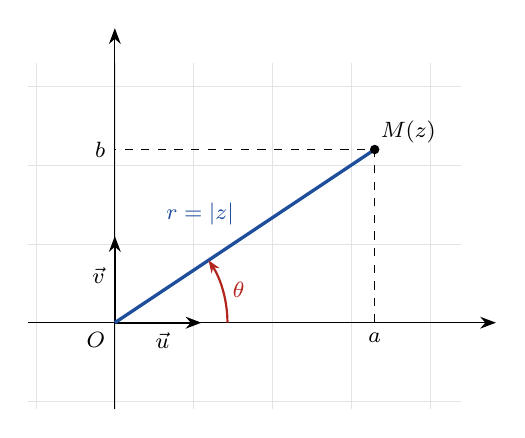
\begin{tikzpicture}[x=1.1cm,y=1.1cm,font=\footnotesize]
 \draw[gray!22,very thin] (-1,-1) grid (4,3);
 \draw[-{Stealth[length=2mm]}] (-1,0)--(4.4,0);
 \draw[-{Stealth[length=2mm]}] (0,-1)--(0,3.4);
 \draw[thick,-{Stealth[length=2mm]}] (0,0)--(1,0) node[pos=0.55,below]{$\vec u$};
 \draw[thick,-{Stealth[length=2mm]}] (0,0)--(0,1) node[pos=0.55,left]{$\vec v$};
 \node[below left] at (0,0){$O$};
 \draw[dashed] (3,0) node[below]{$a$}--(3,2)--(0,2) node[left]{$b$};
 \draw[very thick,cDef] (0,0)--(3,2) node[pos=0.5,above left]{$r=|z|$};
 \draw[cThm,thick,-{Stealth[length=1.6mm]}] (1.3,0) arc (0:33.69:1.3) node[pos=0.5,right]{$\theta$};
 \Pt{3,2}{M(z)}
\end{tikzpicture}\end{LTR}\end{center}

\begin{khassia}[خواص العمدة]
من أجل كل عددين مركبين غير معدومين $z$ و$z'$ ومن أجل كل عدد طبيعي $n$ (بتقدير $2k\pi$):
\[\arg(zz')=\arg z+\arg z'\ ;\quad \arg\Big(\frac{z}{z'}\Big)=\arg z-\arg z'\ ;\quad \arg\Big(\frac{1}{z}\Big)=-\arg z\ ;\quad \arg(z^n)=n\arg z\]
\[\arg(\overline{z})=-\arg z\ ;\qquad \arg(-z)=\pi+\arg z\]
\begin{itemize}
\item $z$ حقيقي موجب تمامًا $\iff\arg z=2k\pi$ \ ؛ \ $z$ حقيقي سالب تمامًا $\iff\arg z=\pi+2k\pi$.
\item $z$ حقيقي غير معدوم $\iff\arg z=k\pi$ \ ؛ \ $z$ تخيلي صرف غير معدوم $\iff\arg z=\dfrac{\pi}{2}+k\pi$.
\end{itemize}
\end{khassia}

\begin{mithal}[طويلات وعمدات يجب حفظها]
\begin{center}
\renewcommand{\arraystretch}{1.6}
\begin{tabular}{|C|c|c|c|c|c|c|c|}\hline
\rowcolor{cSec!12} $z$ & $1$ & $i$ & $-1$ & $-i$ & $1+i$ & $1+i\sqrt3$ & $\sqrt3+i$\\\hline
$|z|$ & $1$ & $1$ & $1$ & $1$ & $\sqrt2$ & $2$ & $2$\\\hline
$\arg z$ & $0$ & $\frac{\pi}{2}$ & $\pi$ & $-\frac{\pi}{2}$ & $\frac{\pi}{4}$ & $\frac{\pi}{3}$ & $\frac{\pi}{6}$\\\hline
\end{tabular}
\end{center}
مثال حساب: $z=-1+i\sqrt3$: \ $r=\sqrt{1+3}=2$ ، \ $\cos\theta=-\dfrac12$ و$\sin\theta=\dfrac{\sqrt3}{2}$ ، إذن $\bx{\arg z=\dfrac{2\pi}{3}+2k\pi}$.
\end{mithal}

%================================================================
\section{الشكل المثلثي، الشكل الأسي ودستور موافر}
\begin{tarif}[الشكل المثلثي والشكل الأسي]
كل عدد مركب غير معدوم $z$ طويلته $r$ وعمدته $\theta$ يُكتب:
\begin{center}\bx{z=r(\cos\theta+i\sin\theta)} \ (الشكل المثلثي)\qquad\qquad \bx{z=re^{i\theta}} \ (الشكل الأسي)\end{center}
حيث نضع اصطلاحًا: $e^{i\theta}=\cos\theta+i\sin\theta$. \ وبالعكس: إذا كان $z=re^{i\theta}$ مع $r>0$ فإن $|z|=r$ و$\arg z=\theta+2k\pi$.
\end{tarif}
\begin{molahada}[انتبه إلى شرط $r>0$]
$z=-2e^{i\frac{\pi}{5}}$ ليس شكلًا أسيًا لأن $-2<0$؛ نكتب $-1=e^{i\pi}$ فيكون $z=2e^{i\pi}e^{i\frac{\pi}{5}}=\bx{2e^{i\frac{6\pi}{5}}}$.
\par وكذلك $z=\cos\theta-i\sin\theta=\cos(-\theta)+i\sin(-\theta)=e^{-i\theta}$.
\end{molahada}

\begin{mithal}[جيب وجيب تمام زوايا شهيرة]
\begin{center}
\renewcommand{\arraystretch}{2.2}
\large\begin{tabular}{|C|c|c|c|c|c|}\hline
\rowcolor{cSec!12} $\theta$ & $0$ & $\dfrac{\pi}{6}$ & $\dfrac{\pi}{4}$ & $\dfrac{\pi}{3}$ & $\dfrac{\pi}{2}$\\\hline
$\cos\theta$ & $1$ & $\dfrac{\sqrt3}{2}$ & $\dfrac{\sqrt2}{2}$ & $\dfrac12$ & $0$\\\hline
$\sin\theta$ & $0$ & $\dfrac12$ & $\dfrac{\sqrt2}{2}$ & $\dfrac{\sqrt3}{2}$ & $1$\\\hline
\end{tabular}
\end{center}
\end{mithal}

\begin{tariqa}[كتابات تشبه الشكل المثلثي وليست كذلك]
الشكل المثلثي هو $r(\cos\theta+i\sin\theta)$ بالضبط مع $r>0$. نستعمل الزوايا المرفقة:
$\cos(-x)=\cos x$ ، $\sin(-x)=-\sin x$ ، $\cos(\pi+x)=-\cos x$ ، $\sin(\pi+x)=-\sin x$ ، $\cos\big(\frac{\pi}{2}-x\big)=\sin x$ ، $\cos\big(\frac{\pi}{2}+x\big)=-\sin x$ ، $\sin\big(\frac{\pi}{2}+x\big)=\cos x$.
\begin{itemize}
\item $4\Big(\cos\dfrac{\pi}{4}-i\sin\dfrac{\pi}{4}\Big)=4\Big(\cos\Big(-\dfrac{\pi}{4}\Big)+i\sin\Big(-\dfrac{\pi}{4}\Big)\Big)=\bx{4e^{-i\frac{\pi}{4}}}$.
\item $-3\Big(\cos\dfrac{\pi}{3}+i\sin\dfrac{\pi}{3}\Big)=3\Big(\cos\Big(\pi+\dfrac{\pi}{3}\Big)+i\sin\Big(\pi+\dfrac{\pi}{3}\Big)\Big)=\bx{3e^{i\frac{4\pi}{3}}}$.
\item $-\sin\dfrac{\pi}{6}+i\cos\dfrac{\pi}{6}=\cos\Big(\dfrac{\pi}{2}+\dfrac{\pi}{6}\Big)+i\sin\Big(\dfrac{\pi}{2}+\dfrac{\pi}{6}\Big)=\bx{e^{i\frac{2\pi}{3}}}$.
\item $\sqrt5\Big(\sin\dfrac{\pi}{6}+i\cos\dfrac{\pi}{6}\Big)=\sqrt5\Big(\cos\dfrac{\pi}{3}+i\sin\dfrac{\pi}{3}\Big)=\bx{\sqrt5\,e^{i\frac{\pi}{3}}}$.
\end{itemize}
\end{tariqa}

\begin{khassia}[قواعد الحساب على الشكل الأسي]
من أجل كل الأعداد الحقيقية $\theta$ و$\theta'$ ومن أجل كل عدد صحيح $n$:
\[e^{i\theta}\times e^{i\theta'}=e^{i(\theta+\theta')}\ ;\quad \frac{e^{i\theta}}{e^{i\theta'}}=e^{i(\theta-\theta')}\ ;\quad \overline{e^{i\theta}}=\frac{1}{e^{i\theta}}=e^{-i\theta}\ ;\quad \big(e^{i\theta}\big)^n=e^{in\theta}\ ;\quad |e^{i\theta}|=1\]
\[e^{i0}=1\ ,\quad e^{i\frac{\pi}{2}}=i\ ,\quad e^{i\pi}=-1\ ,\quad e^{-i\frac{\pi}{2}}=-i\]
\begin{center}$re^{i\theta}=r'e^{i\theta'}\iff$ \bxt{$r=r'$ و $\theta=\theta'+2k\pi$} \quad ($r>0$ و $r'>0$)\end{center}
\end{khassia}

\begin{khassia}[دستور موافر ودستورا أولر]
من أجل كل عدد حقيقي $\theta$ ومن أجل كل عدد طبيعي $n$:
\begin{center}\bx{(\cos\theta+i\sin\theta)^n=\cos(n\theta)+i\sin(n\theta)} \quad (دستور موافر)\end{center}
\begin{center}\bx{\cos\theta=\frac{e^{i\theta}+e^{-i\theta}}{2}}\qquad \bx{\sin\theta=\frac{e^{i\theta}-e^{-i\theta}}{2i}} \quad (دستورا أولر)\end{center}
\end{khassia}

\begin{tariqa}[متى يكون $z^n$ حقيقيًا أو تخيليًا صرفًا؟]
نكتب $z=re^{i\theta}$ فيكون $z^n=r^ne^{in\theta}$، و$n$ عدد طبيعي:
\begin{itemize}
\item $z^n$ حقيقي $\iff n\theta=k\pi$ \ ؛ \ حقيقي موجب $\iff n\theta=2k\pi$ \ ؛ \ حقيقي سالب $\iff n\theta=\pi+2k\pi$.
\item $z^n$ تخيلي صرف $\iff n\theta=\dfrac{\pi}{2}+k\pi$.
\item $z^n$ تخيلي صرف جزؤه التخيلي موجب $\iff n\theta=\dfrac{\pi}{2}+2k\pi$ \ ؛ \ سالب $\iff n\theta=-\dfrac{\pi}{2}+2k\pi$.
\end{itemize}
ثم نعبر عن $n$ بدلالة $k$ ونحتفظ بالقيم الطبيعية فقط.
\end{tariqa}

\begin{mithal}[$z=1+i$]
\begin{itemize}
\item $|z|=\sqrt2$ و$\cos\theta=\sin\theta=\dfrac{\sqrt2}{2}$، إذن:
\[z=\sqrt2\Big(\cos\frac{\pi}{4}+i\sin\frac{\pi}{4}\Big)=\bx{\sqrt2\,e^{i\frac{\pi}{4}}}\qquad;\qquad z^n=(\sqrt2)^n e^{i\frac{n\pi}{4}}\]
\item $z^n$ حقيقي $\iff\dfrac{n\pi}{4}=k\pi\iff \bx{n=4k\ ,\ k\in\N}$.
\item $z^n$ تخيلي صرف $\iff\dfrac{n\pi}{4}=\dfrac{\pi}{2}+k\pi\iff \bx{n=4k+2\ ,\ k\in\N}$.
\item $2026=4\times506+2$ إذن $z^{2026}$ تخيلي صرف:
\[z^{2026}=(\sqrt2)^{2026}e^{i\frac{2026\pi}{4}}=2^{1013}e^{i\left(126\times2\pi+\frac{\pi}{2}\right)}=2^{1013}e^{i\frac{\pi}{2}}=\bx{2^{1013}\,i}\]
\end{itemize}
\end{mithal}

\begin{mithal}[استنتاج قيم مضبوطة لـ $\cos\frac{\pi}{12}$ و$\sin\frac{\pi}{12}$]
نضع $Z=\dfrac{1+i\sqrt3}{1+i}$.
\begin{itemize}
\item الشكل الأسي: \quad $Z=\dfrac{2e^{i\frac{\pi}{3}}}{\sqrt2\,e^{i\frac{\pi}{4}}}=\sqrt2\,e^{i\left(\frac{\pi}{3}-\frac{\pi}{4}\right)}=\sqrt2\,e^{i\frac{\pi}{12}}=\sqrt2\cos\dfrac{\pi}{12}+i\sqrt2\sin\dfrac{\pi}{12}$.
\item الشكل الجبري: \quad $Z=\dfrac{(1+i\sqrt3)(1-i)}{(1+i)(1-i)}=\dfrac{1+\sqrt3}{2}+i\,\dfrac{\sqrt3-1}{2}$.
\item بمطابقة الجزأين الحقيقيين والتخيليين:
\end{itemize}
\begin{center}\bx{\cos\frac{\pi}{12}=\frac{\sqrt6+\sqrt2}{4}} \qquad و\qquad \bx{\sin\frac{\pi}{12}=\frac{\sqrt6-\sqrt2}{4}}\end{center}
\end{mithal}

%================================================================
\origNeedspace{22\baselineskip}
\section{المعادلات في $\mathbb{C}$}
\subsection{معادلات من الدرجة الأولى}
\begin{tariqa}
\begin{itemize}
\item $az=b$ مع $a\neq0$: \ $z=\dfrac{b}{a}$ ثم نكتبه على الشكل الجبري (الضرب في مرافق المقام).
\item معادلة تحوي $z$ و$\overline{z}$: نضع $z=x+iy$ ثم نطابق الجزأين الحقيقيين والتخيليين.
\end{itemize}
\end{tariqa}
\begin{mithal}
$(1+i)z=3-i\iff z=\dfrac{3-i}{1+i}=\bx{1-2i}$ \quad (أنظر الفقرة 2).
\end{mithal}

\subsection{معادلات من الدرجة الثانية بمعاملات حقيقية}
\begin{khassia}[حل $az^2+bz+c=0$ \ ($a,b,c$ حقيقية، $a\neq0$)]
نحسب المميز $\Delta=b^2-4ac$:
\begin{itemize}
\item $\Delta>0$: حلان حقيقيان \quad $z_1=\dfrac{-b-\sqrt\Delta}{2a}$ \ و\ $z_2=\dfrac{-b+\sqrt\Delta}{2a}$.
\item $\Delta=0$: حل مضاعف حقيقي \quad $z_0=-\dfrac{b}{2a}$.
\item $\Delta<0$: حلان مركبان مترافقان \quad $\bx{z_1=\dfrac{-b-i\sqrt{-\Delta}}{2a}}$ \ و\ $\bx{z_2=\overline{z_1}=\dfrac{-b+i\sqrt{-\Delta}}{2a}}$
\end{itemize}
في كل الحالات: $az^2+bz+c=a(z-z_1)(z-z_2)$ ، \ $z_1+z_2=-\dfrac{b}{a}$ \ و\ $z_1z_2=\dfrac{c}{a}$.
\par حالة خاصة: $z^2=d$ مع $d<0$: \ $z=i\sqrt{-d}$ أو $z=-i\sqrt{-d}$ \ (مثلًا $z^2=-9\iff z=3i$ أو $z=-3i$).
\end{khassia}
\begin{mithal}
$z^2-2z+5=0$: \ $\Delta=4-20=-16=(4i)^2$ ، إذن $z_1=\dfrac{2-4i}{2}=\bx{1-2i}$ \ و\ $z_2=\bx{1+2i}$.
\end{mithal}

\begin{mithal}[معادلة بوسيط]
$z^2-2(\cos\theta)z+1=0$ حيث $\theta\in\R$: \ $\Delta=4\cos^2\theta-4=-4\sin^2\theta=(2i\sin\theta)^2$،
ومنه الحلان: $z=\cos\theta-i\sin\theta=\bx{e^{-i\theta}}$ \ و\ $z=\cos\theta+i\sin\theta=\bx{e^{i\theta}}$.
\end{mithal}

\subsection{الجذران التربيعيان لعدد مركب \ (شعبة علوم تجريبية)}
\begin{tariqa}[حل $w^2=a+ib$]
كل عدد مركب غير معدوم له جذران تربيعيان متناقضان. نضع $w=x+iy$؛ من $w^2=a+ib$ و$|w|^2=|a+ib|$:
\[\begin{cases}x^2+y^2=\sqrt{a^2+b^2}\\ x^2-y^2=a\\ 2xy=b\end{cases}\]
نجمع ونطرح المعادلتين الأوليين لإيجاد $x^2$ و$y^2$، ثم نختار الإشارات بحيث يكون $xy$ من نفس إشارة $b$.
\end{tariqa}
\begin{mithal}
الجذران التربيعيان لـ $8+6i$:
\begin{itemize}
\item $x^2+y^2=\sqrt{64+36}=10$ \ ، \ $x^2-y^2=8$ \ ، \ $xy=3>0$.
\item بالجمع: $2x^2=18$ أي $x^2=9$؛ وبالطرح: $2y^2=2$ أي $y^2=1$.
\item $x$ و$y$ من نفس الإشارة (لأن $xy>0$)، إذن: \ \bx{w=3+i} \ أو \ \bx{w=-3-i}.
\item تحقق: $(3+i)^2=9+6i+i^2=8+6i$ \ok.
\end{itemize}
\end{mithal}

\subsection{معادلات تؤول إلى الدرجة الثانية: الدرجة الثالثة بجذر معلوم}
\begin{tariqa}
لحل $P(z)=0$ حيث $P(z)=az^3+bz^2+cz+d$:
\begin{enumerate}
\item نتحقق أن $P(z_0)=0$ (الجذر معطى أو يُخمَّن: $1$، $-1$، $2$، $i$، $\ldots$).
\item نكتب $P(z)=(z-z_0)(\alpha z^2+\beta z+\gamma)$ وننشر ثم نطابق المعاملات (أو نستعمل القسمة الإقليدية / طريقة هورنر).
\item نحل المعادلة من الدرجة الثانية $\alpha z^2+\beta z+\gamma=0$.
\end{enumerate}
\end{tariqa}
\begin{mithal}
$P(z)=z^3+z^2-4z+6$. \ $P(-3)=-27+9+12+6=0$ إذن $-3$ جذر لـ $P$.
\par نكتب $P(z)=(z+3)(\alpha z^2+\beta z+\gamma)=\alpha z^3+(\beta+3\alpha)z^2+(\gamma+3\beta)z+3\gamma$.
بالمطابقة: $\alpha=1$ ، $\beta+3=1$ ، $3\gamma=6$ ، أي $\alpha=1$ ، $\beta=-2$ ، $\gamma=2$:
\[P(z)=(z+3)(z^2-2z+2)\]
$z^2-2z+2=0$: \ $\Delta=-4=(2i)^2$ ، حلاها $1-i$ و$1+i$. \quad إذن حلول $P(z)=0$ هي: \bx{-3\ ;\ 1-i\ ;\ 1+i}.
\end{mithal}
%================================================================
\section{التفسير الهندسي للأعداد المركبة}
\begin{khassia}[المسافات والزوايا]
$A$ ، $B$ ، $C$ ، $D$ نقط لواحقها $z_A$ ، $z_B$ ، $z_C$ ، $z_D$ ، مع $A\neq B$ و$C\neq D$:
\[\bx{AB=|z_B-z_A|}\qquad \bx{(\vec u;\overrightarrow{AB})=\arg(z_B-z_A)+2k\pi}\]
\[\bx{(\overrightarrow{AB};\overrightarrow{CD})=\arg\Big(\frac{z_D-z_C}{z_B-z_A}\Big)+2k\pi}\qquad;\qquad \bx{(\overrightarrow{AB};\overrightarrow{AC})=\arg\Big(\frac{z_C-z_A}{z_B-z_A}\Big)+2k\pi}\]
\end{khassia}

\begin{khassia}[الاستقامية والتعامد]
نضع $L=\dfrac{z_C-z_A}{z_B-z_A}$ \ ($A\neq B$):
\begin{itemize}
\item $A$ ، $B$ ، $C$ في استقامية $\iff L$ عدد حقيقي $\iff \arg L=k\pi$ (إذا كان $C\neq A$).
\item $(AB)\perp(AC)\iff L$ عدد تخيلي صرف غير معدوم $\iff \arg L=\dfrac{\pi}{2}+k\pi$.
\item بصفة عامة: $(AB)\parallel(CD)\iff\dfrac{z_D-z_C}{z_B-z_A}\in\R$ \ و\ $(AB)\perp(CD)\iff\dfrac{z_D-z_C}{z_B-z_A}$ تخيلي صرف.
\end{itemize}
\end{khassia}

\begin{khassia}[طبيعة المثلث $ABC$ انطلاقًا من $L=\dfrac{z_C-z_A}{z_B-z_A}$]
\begin{itemize}
\item $|L|=1$ \ ($AC=AB$): المثلث متساوي الساقين رأسه $A$.
\item $\arg L=\pm\dfrac{\pi}{2}+2k\pi$: المثلث قائم في $A$.
\item $L=i$ أو $L=-i$ \ ($|L|=1$ و$\arg L=\pm\frac{\pi}{2}$): المثلث قائم ومتساوي الساقين في $A$.
\item $L=e^{i\frac{\pi}{3}}$ أو $L=e^{-i\frac{\pi}{3}}$: المثلث متقايس الأضلاع.
\end{itemize}
\end{khassia}

\begin{khassia}[الرباعيات والنقط المتداورة]
\begin{itemize}
\item $ABCD$ متوازي أضلاع $\iff z_B-z_A=z_C-z_D\iff\dfrac{z_A+z_C}{2}=\dfrac{z_B+z_D}{2}$ (منتصفا القطرين منطبقان).
\item متوازي أضلاع قطراه متعامدان: معين ؛ قطراه متقايسان ($AC=BD$): مستطيل ؛ قطراه متعامدان ومتقايسان: مربع.
\item متوازي أضلاع $ABCD$ يكون: معينًا إذا كان $AB=AD$، مستطيلًا إذا كان $(AB)\perp(AD)$، مربعًا إذا كان $\dfrac{z_D-z_A}{z_B-z_A}=\pm i$.
\item النقط $A$ ، $B$ ، $C$ ، $D$ تنتمي إلى دائرة مركزها $\Omega$ $\iff |z_A-z_\Omega|=|z_B-z_\Omega|=|z_C-z_\Omega|=|z_D-z_\Omega|$.
\end{itemize}
\end{khassia}

\begin{mithal}[طبيعة مثلث ورباعي]
$A(1+i)$ ، $B(3+2i)$ ، $C(3i)$.
\[L=\frac{z_C-z_A}{z_B-z_A}=\frac{-1+2i}{2+i}=\frac{(-1+2i)(2-i)}{(2+i)(2-i)}=\frac{-2+i+4i-2i^2}{5}=\frac{5i}{5}=\bx{i}\]
$|L|=1$ و$\arg L=\dfrac{\pi}{2}$ إذن \bxt{المثلث $ABC$ قائم ومتساوي الساقين في $A$}.
\par النقطة $D$ بحيث $ABDC$ متوازي أضلاع: $z_D=z_B+z_C-z_A=\bx{2+4i}$. ولأن $AB=AC$ و$(AB)\perp(AC)$ فإن \bxt{$ABDC$ مربع}.
\par مركز المربع: $\Omega$ منتصف $[AD]$، $z_\Omega=\dfrac32+\dfrac52 i$؛ والنقط $A$ ، $B$ ، $D$ ، $C$ تنتمي إلى الدائرة التي مركزها $\Omega$ ونصف قطرها $\Omega A=\Big|{-\dfrac12}-\dfrac32 i\Big|=\dfrac{\sqrt{10}}{2}$.
\begin{CP}{-1}{4}{-1}{5}{0.9}
 \draw[cEx,thick,dashed] (1.5,2.5) circle ({sqrt(10)/2});
 \fill[cDef!10] (1,1)--(3,2)--(2,4)--(0,3)--cycle;
 \draw[cDef,very thick] (1,1)--(3,2)--(2,4)--(0,3)--cycle;
 \draw[cDef] (1,1)++(0.4,0.2)--++(-0.2,0.4)--++(-0.4,-0.2);
 \path (1,1)--(3,2) node[midway,sloped,cThm]{$|$};
 \path (1,1)--(0,3) node[midway,sloped,cThm]{$|$};
 \Pt[below]{1,1}{A} \Pt[right]{3,2}{B} \Pt[above]{2,4}{D} \Pt[left]{0,3}{C} \Pt[right]{1.5,2.5}{\Omega}
\end{CP}
\end{mithal}

%================================================================
\section{مجموعات النقط}
\begin{khassia}[مجموعات النقط الأساسية]
$M$ نقطة لاحقتها $z$ ، و$A$ ، $B$ نقطتان متمايزتان، $r>0$ و$\theta$ عدد حقيقي:
\begin{itemize}
\item $|z-z_A|=r\iff AM=r$: \quad $M$ تنتمي إلى \bxt{الدائرة التي مركزها $A$ ونصف قطرها $r$}.
\item $z=z_A+re^{i\alpha}$ حيث $\alpha$ يمسح $\R$: \quad نفس الدائرة.
\item $|z-z_A|=|z-z_B|\iff MA=MB$: \quad $M$ تنتمي إلى \bxt{محور القطعة $[AB]$}.
\item $\arg(z-z_A)=\theta+2k\pi$: \quad \bxt{نصف المستقيم الذي مبدؤه $A$ وشعاع توجيهه $\vec w(e^{i\theta})$ ما عدا $A$}.
\item $\arg(z-z_A)=\theta+k\pi$: \quad \bxt{المستقيم المار بـ $A$ وشعاع توجيهه $\vec w(e^{i\theta})$ ما عدا $A$}.
\item $\dfrac{z-z_A}{z-z_B}$ حقيقي: \quad \bxt{المستقيم $(AB)$ ما عدا $B$}.
\item $\dfrac{z-z_A}{z-z_B}$ تخيلي صرف: \quad $(\overrightarrow{MA}\perp\overrightarrow{MB})$: \bxt{الدائرة التي قطرها $[AB]$ ما عدا $B$}.
\item $\arg\Big(\dfrac{z_B-z}{z_A-z}\Big)=\pi+2k\pi$: \quad $(\overrightarrow{MA};\overrightarrow{MB})=\pi$: \bxt{القطعة $]AB[$}.
\item $\arg\Big(\dfrac{z_B-z}{z_A-z}\Big)=2k\pi$: \quad \bxt{المستقيم $(AB)$ ما عدا القطعة $[AB]$}.
\item $\arg\Big(\dfrac{z_B-z}{z_A-z}\Big)=\dfrac{\pi}{2}+2k\pi$ (أو $-\dfrac{\pi}{2}+2k\pi$): \quad \bxt{نصف دائرة قطرها $[AB]$ ما عدا $A$ و$B$}.
\item $z=z_A+ke^{i\theta}$ ($\theta$ ثابت): $k$ يمسح $\R_+^*$: \bxt{نصف مستقيم مبدؤه $A$ ما عدا $A$} ؛ $k$ يمسح $\R$: \bxt{مستقيم يشمل $A$}.
\item $(z-z_A)(\overline{z}-\overline{z_A})=r^2\iff|z-z_A|^2=r^2$: \quad دائرة مركزها $A$ ونصف قطرها $r$.
\end{itemize}
\end{khassia}

\begin{tariqa}[تعيين مجموعة نقط]
\begin{enumerate}
\item نكتب الشرط على شكل مسافات $|z-z_A|=MA$ أو زوايا $\arg(z-z_A)=(\vec u;\overrightarrow{AM})$ ثم نتعرف على المجموعة.
\item إذا تعذر ذلك نضع $z=x+iy$ ونبحث عن معادلة ديكارتية: $(x-x_0)^2+(y-y_0)^2=r^2$ دائرة، $ax+by+c=0$ مستقيم.
\item ننتبه إلى النقط المستثناة (حيث العمدة غير معرفة أو المقام معدوم).
\end{enumerate}
\end{tariqa}

\begin{khassia}[مجموعات نقط بالمرجح]
إذا كان $G$ مرجح $\{(A;\alpha),(B;\beta),(C;\gamma)\}$ مع $\alpha+\beta+\gamma\neq0$ فإن:
$\alpha\overrightarrow{MA}+\beta\overrightarrow{MB}+\gamma\overrightarrow{MC}=(\alpha+\beta+\gamma)\overrightarrow{MG}$.
\par ومنه: $\|\alpha\overrightarrow{MA}+\beta\overrightarrow{MB}+\gamma\overrightarrow{MC}\|=k\iff MG=\dfrac{k}{|\alpha+\beta+\gamma|}$: \ دائرة مركزها $G$.
\end{khassia}

\begin{mithal}[ثلاث مجموعات في شكل واحد]
\begin{itemize}
\item $(E_1)$: $|z-2-i|=2\iff|z-(2+i)|=2$: \ \bxt{الدائرة التي مركزها $I(2+i)$ ونصف قطرها $2$}.
\item $(E_2)$: $|z+1|=|z-i|\iff MA=MB$ مع $A(-1)$ و$B(i)$: \ \bxt{محور $[AB]$}.
بوضع $z=x+iy$: \ $(x+1)^2+y^2=x^2+(y-1)^2\iff 2x+1=-2y+1\iff \bx{y=-x}$.
\item $(E_3)$: $\arg(z-1)=\dfrac{\pi}{4}+2k\pi$ مع $C(1)$: \ \bxt{نصف المستقيم الذي مبدؤه $C$ ويوازي $\vec u+\vec v$ ما عدا $C$}.
\end{itemize}
\begin{CP}{-3}{5}{-2}{4}{0.9}
 \draw[cDef,very thick] (2,1) circle (2);
 \draw[cThm,very thick] (-3,3)--(2,-2);
 \draw[cRem,very thick,-{Stealth[length=2.5mm]}] (1,0)--(4,3);
 \draw[cRem,fill=white,thick] (1,0) circle (2.2pt);
 \draw[cRem] (1.6,0) arc (0:45:0.6) node[midway,right,font=\scriptsize]{$\frac{\pi}{4}$};
 \fill (2,1) circle (1.7pt) node[above right]{$I$};
 \Pt[above left]{-1,0}{A} \Pt[above left]{0,1}{B}
 \node[cRem,below right] at (1,0){$C$};
 \node[cDef,right] at (3.6,-0.4){$(E_1)$};
 \node[cThm,right] at (2,-2){$(E_2)$};
 \node[cRem,above] at (4,3){$(E_3)$};
\end{CP}
\end{mithal}

%================================================================
\section{التحويلات النقطية}
\subsection{الكتابة المركبة لتحويل نقطي}
\begin{tarif}
تحويل نقطي $F$ يرفق بكل نقطة $M(z)$ نقطة $M'(z')$. \textbf{الكتابة المركبة} لـ $F$ هي العلاقة التي تعطي $z'$ بدلالة $z$.
\par \textbf{نقطة صامدة}: $F(\Omega)=\Omega$. \ للتحويل $z'=az+b$ مع $a\neq1$ نقطة صامدة وحيدة لاحقتها \quad $\bx{\omega=\dfrac{b}{1-a}}$ \quad (حل $z=az+b$)،
وتصبح الكتابة: \quad $\bx{z'-\omega=a(z-\omega)}$
\end{tarif}

\subsection{الانسحاب، التحاكي، الدوران}
\begin{khassia}[الانسحاب]
الانسحاب الذي شعاعه $\vec w$ ذو اللاحقة $b$: \quad $\overrightarrow{MM'}=\vec w\iff \bx{z'=z+b}$.
\end{khassia}
\begin{khassia}[التحاكي]
التحاكي الذي مركزه $\Omega(\omega)$ ونسبته $k$ (حقيقي غير معدوم): \quad $\overrightarrow{\Omega M'}=k\overrightarrow{\Omega M}\iff \bx{z'-\omega=k(z-\omega)}$.
\par يضرب المسافات في $|k|$ والمساحات في $k^2$.
\end{khassia}
\begin{khassia}[الدوران]
الدوران الذي مركزه $\Omega(\omega)$ وزاويته $\theta$:
\[\begin{cases}\Omega M'=\Omega M\\ (\overrightarrow{\Omega M};\overrightarrow{\Omega M'})=\theta+2k\pi\end{cases}\ (M\neq\Omega)\iff \bx{z'-\omega=e^{i\theta}(z-\omega)}\]
يحافظ على المسافات والزوايا الموجهة. \ دوران زاويته $\dfrac{\pi}{2}$: $z'-\omega=i(z-\omega)$ ؛ \ زاويته $\pi$: تناظر مركزي.
\end{khassia}

\begin{center}\begin{LTR}\begin{tikzpicture}[font=\footnotesize]
 % translation
 \begin{scope}[xshift=11.2cm]
 \draw[cDef,very thick,-{Stealth[length=2.5mm]}] (0,0)--(1.8,0.9) node[midway,above left]{$\vec w$};
 \Pt[below]{0,0}{M} \Pt[right]{1.8,0.9}{M'}
 \node[cSec] at (0.9,-1.4){\ar{\textbf{انسحاب}}};
 \end{scope}
 % homothety
 \begin{scope}[xshift=7.4cm]
 \draw[thick,cThm] (0,0)--(2.4,1.2);
 \Pt[below]{0,0}{\Omega} \Pt[below right]{1.2,0.6}{M} \Pt[right]{2.4,1.2}{M'}
 \node[cThm,above,font=\scriptsize] at (1.0,1.15){$\overrightarrow{\Omega M'}=2\,\overrightarrow{\Omega M}$};
 \node[cSec] at (1.2,-1.4){\ar{\textbf{تحاك}}};
 \end{scope}
 % rotation
 \begin{scope}[xshift=3.9cm]
 \draw[thick,cRem] (0,0)--(1.6,0) (0,0)--(60:1.6);
 \draw[cRem,-{Stealth[length=2mm]}] (0.6,0) arc (0:60:0.6) node[midway,right]{$\theta$};
 \path (0,0)--(1.6,0) node[midway,sloped]{$|$};
 \path (0,0)--(60:1.6) node[midway,sloped]{$|$};
 \Pt[below]{0,0}{\Omega} \Pt[right]{1.6,0}{M} \Pt[above]{60:1.6}{M'}
 \node[cSec] at (0.8,-1.4){\ar{\textbf{دوران}}};
 \end{scope}
 % similitude
 \begin{scope}
 \draw[thick,cMeth] (0,0)--(1.2,0)--(1.2,1.2)--cycle;
 \draw[cMeth] (1.0,0)--(1.0,0.2)--(1.2,0.2);
 \draw[cMeth,-{Stealth[length=2mm]}] (0.55,0) arc (0:45:0.55) node[midway,right,font=\scriptsize]{$\frac{\pi}{4}$};
 \Pt[below]{0,0}{\Omega} \Pt[below right]{1.2,0}{M} \Pt[above]{1.2,1.2}{M'}
 \node[cMeth,right,font=\scriptsize] at (1.3,0.6){$\Omega M'=\sqrt2\,\Omega M$};
 \node[cSec] at (0.9,-1.4){\ar{\textbf{تشابه مباشر}}};
 \end{scope}
\end{tikzpicture}\end{LTR}\end{center}

\subsection{التشابه المباشر \ (رياضيات، تقني رياضي، علوم تجريبية)}
\begin{tarif}[التشابه المباشر]
التحويل النقطي ذو الكتابة المركبة $\bx{z'=az+b}$ حيث $a\in\mathbb{C}^*$ و$b\in\mathbb{C}$ يسمى \textbf{تشابهًا مباشرًا}.
إذا كان $a\neq1$ فإن له مركزًا $\Omega(\omega)$ مع $\omega=\dfrac{b}{1-a}$، و:
\begin{itemize}
\item \textbf{نسبته} $k=|a|$ \ و\ \textbf{زاويته} $\theta=\arg a$: \quad $\bx{z'-\omega=ke^{i\theta}(z-\omega)}$
\item من أجل $M\neq\Omega$: \ $\Omega M'=k\,\Omega M$ \ و\ $(\overrightarrow{\Omega M};\overrightarrow{\Omega M'})=\theta+2k\pi$.
\item إذا كان $a=1$ فهو انسحاب. الانسحاب والتحاكي والدوران حالات خاصة من التشابه المباشر.
\item \textbf{حالة خاصة -- التقايسات}: إذا كان $|a|=1$ فإن $S$ يحافظ على المسافات ($M'N'=MN$): هو انسحاب ($a=1$) أو دوران ($a\neq1$).
\end{itemize}
\end{tarif}
\begin{khassia}[خواص التشابه المباشر $S$ ذي النسبة $k$ والزاوية $\theta$]
\begin{itemize}
\item إذا كانت $S(M)=M'$ و$S(N)=N'$ فإن: \ $M'N'=k\,MN$ \ و\ $(\overrightarrow{MN};\overrightarrow{M'N'})=\theta+2k\pi$؛ ويضرب المساحات في $k^2$.
\item يحافظ على الاستقامية، التوازي، التعامد، الزوايا الموجهة والمرجح (المنتصف).
\item صورة مستقيم مستقيم، وصورة الدائرة $\mathcal{C}(I;R)$ هي الدائرة $\mathcal{C}(S(I);kR)$.
\item يوجد تشابه مباشر وحيد يحول $A$ إلى $A'$ و$B$ إلى $B'$ ($A\neq B$ و$A'\neq B'$): \ $a=\dfrac{z_{B'}-z_{A'}}{z_B-z_A}$ \ و\ $b=z_{A'}-az_A$.
\end{itemize}
\end{khassia}

\begin{khassia}[تركيب تحويلين]
إذا كان $F_1: z'=a_1z+b_1$ و$F_2: z'=a_2z+b_2$ فإن $F_2\circ F_1: z'=a_2(a_1z+b_1)+b_2=\bx{a_1a_2\,z+a_2b_1+b_2}$:
النسبة $|a_1a_2|=k_1k_2$ والزاوية $\theta_1+\theta_2$.
\end{khassia}

\subsection{التحليل القانوني لتشابه مباشر}
\begin{khassia}[التحليل القانوني]
$S$ تشابه مباشر ليس انسحابًا، مركزه $\Omega(\omega)$ ، نسبته $k$ وزاويته $\theta$. نسمي $r$ الدوران الذي مركزه $\Omega$ وزاويته $\theta$ ، و$h$ التحاكي الذي مركزه $\Omega$ ونسبته $k$:
\[\bx{S=h\circ r=r\circ h}\]
وهي كتابة وحيدة لـ $S$ كمركب دوران وتحاكٍ نسبته موجبة لهما نفس المركز $\Omega$. \ البرهان: $r: z_1-\omega=e^{i\theta}(z-\omega)$ و$h: z'-\omega=k(z_1-\omega)$ ، إذن $h\circ r: z'-\omega=ke^{i\theta}(z-\omega)$ ، وبنفس الطريقة $r\circ h$.
\begin{itemize}
\item $k=1$: $S=r$ (دوران) ؛ \ $\theta=0$: $S=h$ (تحاك) ؛ \ $\theta=\pi$: $S$ تحاك نسبته $-k$.
\item \textbf{توظيفه}: لإنشاء $M'=S(M)$ ندير $M$ حول $\Omega$ بزاوية $\theta$ فنحصل على $M_1$ ، ثم $\overrightarrow{\Omega M'}=k\,\overrightarrow{\Omega M_1}$.
\end{itemize}
\end{khassia}
\begin{mithal}[التحليل القانوني]
$S: z'=(1+i\sqrt3)z-i\sqrt3$. \ $a=1+i\sqrt3=2e^{i\frac{\pi}{3}}$ ، \ $\omega=\dfrac{-i\sqrt3}{1-(1+i\sqrt3)}=\dfrac{-i\sqrt3}{-i\sqrt3}=1$.
\begin{itemize}
\item \bxt{$S$ تشابه مباشر مركزه $\Omega(1)$ ، نسبته $2$ وزاويته $\frac{\pi}{3}$} ، \ وتحليله القانوني $S=h\circ r$ حيث:
\[r:\ z'-1=e^{i\frac{\pi}{3}}(z-1)\qquad;\qquad h:\ z'-1=2(z-1)\]
\item صورة $O$: \ $r(O)=O_1$: $z_{O_1}=1-e^{i\frac{\pi}{3}}=\dfrac12-\dfrac{\sqrt3}{2}i$ ، \ ثم $h(O_1)$: $1+2\Big(-\dfrac12-\dfrac{\sqrt3}{2}i\Big)=\bx{-i\sqrt3}$.
\item تحقق مباشر: $z_{S(O)}=(1+i\sqrt3)\times0-i\sqrt3=-i\sqrt3$ \ok. \ المثلث $\Omega OO_1$ متقايس الأضلاع (دوران بزاوية $\frac{\pi}{3}$) و$O_1$ منتصف $[\Omega O']$.
\end{itemize}
\begin{CP}{-1}{2}{-2}{1}{1.3}
 \fill[cEx!12] (1,0)--(0,0)--(0.5,-0.866)--cycle;
 \draw[cEx,thick] (1,0)--(0,0)--(0.5,-0.866)--cycle;
 \draw[cMeth,thick,dashed] (1,0)--(0,-1.732);
 \draw[cEx,-{Stealth[length=2mm]}] (0.6,0) arc (180:240:0.4) node[midway,left,font=\scriptsize]{$\frac{\pi}{3}$};
 \Pt[above]{1,0}{\Omega} \Pt[above left]{0,0}{O} \Pt[right]{0.5,-0.866}{O_1} \Pt[left]{0,-1.732}{O'}
\end{CP}
\end{mithal}

\subsection{التعرف على تحويل انطلاقًا من $z'=az+b$}
\begin{BOX}{cMeth}{جدول التعرف على التحويل}
\begin{center}
\renewcommand{\arraystretch}{1.5}
\begin{tabular}{|p{0.42\textwidth}|p{0.18\textwidth}|p{0.27\textwidth}|}\hline
\rowcolor{cSec!12} \textbf{العناصر المميزة} & \textbf{الشرط على $a$} & \textbf{التحويل}\\\hline
شعاعه $\vec w(b)$ & $a=1$ & انسحاب\\\hline
مركزه $\omega=\frac{b}{1-a}$ ، نسبته $k=a$ & $a\in\R\setminus\{0;1\}$ & تحاك\\\hline
مركزه $\omega=\frac{b}{1-a}$ ، زاويته $\theta=\arg a$ & $|a|=1$ و $a\neq1$ & دوران\\\hline
مركزه $\omega=\frac{b}{1-a}$ ، نسبته $|a|$ ، زاويته $\arg a$ & $a\in\mathbb{C}\setminus\R$ & تشابه مباشر\\\hline
\end{tabular}
\end{center}
\end{BOX}

\begin{mithal}[التعرف على التحويلات]
\begin{itemize}
\item $z'=z+2-i$: \ انسحاب شعاعه $\vec w(2-i)$.
\item $z'=-2z+3$: \ $a=-2\in\R$، $\omega=\dfrac{3}{1+2}=1$: \ \bxt{تحاك مركزه $\Omega(1)$ ونسبته $-2$}.
\item $z'=iz+1+i$: \ $|i|=1$، $\omega=\dfrac{1+i}{1-i}=\dfrac{(1+i)^2}{2}=i$: \ \bxt{دوران مركزه $\Omega(i)$ وزاويته $\frac{\pi}{2}$}.
\par صورة $A(2)$: $z_{A'}=2i+1+i=1+3i$ ، \ وتحقق: $\Omega A=|2-i|=\sqrt5=|1+2i|=\Omega A'$.
\item الدوران الذي مركزه $\Omega(1+i)$ وزاويته $\dfrac{\pi}{3}$: \ $z'=e^{i\frac{\pi}{3}}\big(z-(1+i)\big)+1+i$.
\end{itemize}
\end{mithal}

\begin{mithal}[تشابه مباشر]
$S: z'=(1+i)z-i$. \ $a=1+i=\sqrt2e^{i\frac{\pi}{4}}\notin\R$ ، \ $\omega=\dfrac{-i}{1-(1+i)}=\dfrac{-i}{-i}=1$:
\begin{center}\bxt{$S$ تشابه مباشر مركزه $\Omega(1)$ ، نسبته $\sqrt2$ وزاويته $\frac{\pi}{4}$}\end{center}
صورة $A(2)$: $z_{A'}=(1+i)2-i=2+i$ ، \ وصورة $M(1+i)$: $z_{M'}=(1+i)^2-i=i$.
\par $\dfrac{z_{A'}-z_A}{z_\Omega-z_A}=\dfrac{i}{-1}=-i$ ، إذن المثلث $\Omega AA'$ قائم ومتساوي الساقين في $A$ (وكذلك $\Omega MM'$ في $M$): \ هذه خاصية كل تشابه نسبته $\sqrt2$ وزاويته $\frac{\pi}{4}$.
\begin{CP}{-1}{3}{-1}{2}{1.2}
 \fill[cMeth!12] (1,0)--(2,0)--(2,1)--cycle;
 \draw[cMeth,thick] (1,0)--(2,0)--(2,1)--cycle;
 \draw[cMeth] (1.85,0)--(1.85,0.15)--(2,0.15);
 \fill[cEx!12] (1,0)--(1,1)--(0,1)--cycle;
 \draw[cEx,thick] (1,0)--(1,1)--(0,1)--cycle;
 \draw[cEx] (1,0.85)--(0.85,0.85)--(0.85,1);
 \draw[cMeth,-{Stealth[length=2mm]}] (1.5,0) arc (0:45:0.5);
 \Pt[below]{1,0}{\Omega} \Pt[below]{2,0}{A} \Pt[right]{2,1}{A'} \Pt[above right]{1,1}{M} \Pt[above left]{0,1}{M'}
\end{CP}
\end{mithal}

%================================================================
\section{تمارين محلولة}
\begin{tmr}
\QQ{1} حل في $\mathbb{C}$ المعادلة: \quad $z^2-2\sqrt3\,z+4=0$.
\QQ{2} في المستوي المنسوب إلى معلم متعامد ومتجانس $(O;\vec u,\vec v)$ نعتبر النقطتين $A$ و$B$ لاحقتاهما $z_A=\sqrt3+i$ و$z_B=\sqrt3-i$.
\begin{sq}
\qa اكتب $z_A$ و$z_B$ على الشكل الأسي.
\qb اكتب $\dfrac{z_A}{z_B}$ على الشكل الأسي ثم استنتج طبيعة المثلث $OAB$.
\qc عيّن قيم العدد الطبيعي $n$ التي يكون من أجلها $(z_A)^n$ حقيقيًا، ثم احسب $(z_A)^6$.
\end{sq}
\QQ{3} $r$ الدوران الذي مركزه $O$ ويحول $B$ إلى $A$. عيّن زاويته وكتابته المركبة، ثم احسب لاحقة $C=r(A)$.
\QQ{4} عيّن مجموعة النقط $M(z)$ بحيث: $|z-\sqrt3-i|=|z-\sqrt3+i|$.
\end{tmr}
\begin{hal}
\QQ{1} $\Delta=(-2\sqrt3)^2-4\times1\times4=12-16=-4=(2i)^2<0$، إذن للمعادلة حلان مركبان مترافقان:
\[z_1=\frac{2\sqrt3-2i}{2}=\bx{\sqrt3-i}\qquad\qquad z_2=\overline{z_1}=\bx{\sqrt3+i}\]
\QQ{2}
\pa $|z_A|=\sqrt{3+1}=2$ ، \ $\cos\theta=\dfrac{\sqrt3}{2}$ و$\sin\theta=\dfrac12$ إذن $\theta=\dfrac{\pi}{6}$: \quad $z_A=\bx{2e^{i\frac{\pi}{6}}}$ ، \ و$z_B=\overline{z_A}=\bx{2e^{-i\frac{\pi}{6}}}$.
\pb $\dfrac{z_A}{z_B}=\dfrac{2e^{i\frac{\pi}{6}}}{2e^{-i\frac{\pi}{6}}}=\bx{e^{i\frac{\pi}{3}}}$. \quad ومنه:
\begin{itemize}
\item $\Big|\dfrac{z_A}{z_B}\Big|=1$ أي $OA=OB$ ؛
\item $(\overrightarrow{OB};\overrightarrow{OA})=\arg\Big(\dfrac{z_A}{z_B}\Big)=\dfrac{\pi}{3}+2k\pi$.
\end{itemize}
مثلث متساوي الساقين زاوية رأسه $\dfrac{\pi}{3}$، إذن \bxt{المثلث $OAB$ متقايس الأضلاع}.
\pc $(z_A)^n=2^ne^{i\frac{n\pi}{6}}$. \ $(z_A)^n$ حقيقي $\iff\dfrac{n\pi}{6}=k\pi\iff \bx{n=6k\ ,\ k\in\N}$.
\[(z_A)^6=2^6e^{i\pi}=\bx{-64}\]
\QQ{3} $r$ دوران مركزه $O$ وزاويته $\theta$: $z'=e^{i\theta}z$. \ $r(B)=A$ يعني $z_A=e^{i\theta}z_B$ أي $e^{i\theta}=\dfrac{z_A}{z_B}=e^{i\frac{\pi}{3}}$:
\begin{center}\bxt{زاوية $r$ هي $\frac{\pi}{3}$} \qquad و\qquad \bx{z'=e^{i\frac{\pi}{3}}z}\end{center}
$z_C=e^{i\frac{\pi}{3}}\times2e^{i\frac{\pi}{6}}=2e^{i\frac{\pi}{2}}=\bx{2i}$.
\QQ{4} $|z-z_A|=|z-z_B|\iff MA=MB$: المجموعة هي محور القطعة $[AB]$. \ $A$ و$B$ متناظرتان بالنسبة إلى محور الفواصل (لاحقتاهما مترافقتان)، إذن \bxt{المجموعة هي محور الفواصل}.
\par لاحظ أن $OA=OB=OC=2$: النقط $A$ ، $B$ ، $C$ تنتمي إلى الدائرة التي مركزها $O$ ونصف قطرها $2$.
\begin{CP}{-2}{3}{-2}{3}{1}
 \draw[cEx,thick,dashed] (0,0) circle (2);
 \draw[cThm,very thick] (-2,0)--(3,0);
 \fill[cDef!12] (0,0)--(1.732,1)--(1.732,-1)--cycle;
 \draw[cDef,very thick] (0,0)--(1.732,1)--(1.732,-1)--cycle;
 \draw[cRem,thick,-{Stealth[length=2mm]}] (1.732,-1) arc (-30:30:2);
 \draw[cRem,thick,-{Stealth[length=2mm]}] (1.732,1) arc (30:90:2);
 \node[cRem,right] at (2.05,0.35){$\frac{\pi}{3}$};
 \Pt[above right]{1.732,1}{A} \Pt[below right]{1.732,-1}{B} \Pt[above left]{0,2}{C}
 \node[cThm,below] at (2.75,0){$(E)$};
\end{CP}
\end{hal}

\begin{tmr}
في المستوي المنسوب إلى معلم متعامد ومتجانس $(O;\vec u,\vec v)$ نعتبر النقط $A$ ، $B$ ، $C$ لواحقها $z_A=1+i$ ، $z_B=3+i$ ، $z_C=3+3i$.
\QQ{1} اكتب $L=\dfrac{z_C-z_A}{z_B-z_A}$ على الشكلين الجبري والأسي. \ احسب $\dfrac{z_C-z_B}{z_A-z_B}$ واستنتج طبيعة المثلث $ABC$.
\QQ{2} عيّن لاحقة النقطة $D$ بحيث يكون $ABCD$ متوازي أضلاع، ثم بيّن أنه مربع.
\QQ{3} $S$ التشابه المباشر الذي مركزه $A$ ويحول $B$ إلى $C$.
\begin{sq}
\qa عيّن نسبة $S$ وزاويته، ثم بيّن أن كتابته المركبة هي $z'=(1+i)z+1-i$.
\qb $(\Gamma)$ الدائرة المحيطة بالمربع $ABCD$. عيّن صورتها $(\Gamma')$ بالتشابه $S$.
\end{sq}
\QQ{4} عيّن مجموعة النقط $M(z)$ بحيث: $|z-1-i|=|z-3-3i|$.
\end{tmr}
\begin{hal}
\QQ{1} $L=\dfrac{(3+3i)-(1+i)}{(3+i)-(1+i)}=\dfrac{2+2i}{2}=\bx{1+i}$ ، \ و$|L|=\sqrt2$ ، $\arg L=\dfrac{\pi}{4}$: \ $L=\bx{\sqrt2\,e^{i\frac{\pi}{4}}}$.
\[\frac{z_C-z_B}{z_A-z_B}=\frac{2i}{-2}=\bx{-i}\]
طويلته $1$ أي $BC=BA$، وعمدته $-\dfrac{\pi}{2}$ أي $(BA)\perp(BC)$: \ \bxt{المثلث $ABC$ قائم ومتساوي الساقين في $B$}.
\QQ{2} $ABCD$ متوازي أضلاع $\iff z_B-z_A=z_C-z_D$، ومنه:
\[z_D=z_A+z_C-z_B=(1+i)+(3+3i)-(3+i)=\bx{1+3i}\]
\par متوازي أضلاع فيه زاوية قائمة ($\widehat{ABC}=\frac{\pi}{2}$) وضلعان متتاليان متقايسان ($BA=BC$)، إذن \bxt{$ABCD$ مربع}.
\QQ{3}
\pa $S$ مركزه $A$، و$S(B)=C$ يعني $z_C-z_A=a(z_B-z_A)$ أي $a=L=\sqrt2\,e^{i\frac{\pi}{4}}$:
\begin{center}\bxt{نسبة $S$ هي $\sqrt2$ وزاويته $\frac{\pi}{4}$}\end{center}
الكتابة: $z'-z_A=(1+i)(z-z_A)$، أي:
\[z'=(1+i)z-(1+i)^2+1+i=(1+i)z-2i+1+i=\bx{(1+i)z+1-i}\]
\pb $(\Gamma)$ مركزها $I$ مركز المربع (منتصف $[AC]$): $z_I=2+2i$، ونصف قطرها $IA=|{-1}-i|=\sqrt2$.
صورتها دائرة مركزها $S(I)$ ونصف قطرها $\sqrt2\times\sqrt2=2$:
\[z_{S(I)}=(1+i)(2+2i)+1-i=4i+1-i=1+3i=z_D\]
إذن \bxt{$(\Gamma')$ هي الدائرة التي مركزها $D$ ونصف قطرها $2$}.
\QQ{4} $|z-z_A|=|z-z_C|\iff MA=MC$: المجموعة هي محور القطعة $[AC]$، وهو حامل القطر الآخر للمربع: \bxt{المستقيم $(BD)$}.
\par تحقق: بوضع $z=x+iy$:
\[(x-1)^2+(y-1)^2=(x-3)^2+(y-3)^2\iff 4x+4y=16\iff \bx{x+y=4}\]
والنقطتان $B(3;1)$ و$D(1;3)$ تحققان هذه المعادلة.
\begin{CP}{-2}{5}{-1}{6}{0.85}
 \draw[cEx,thick,dashed] (1,3) circle (2);
 \draw[cDef,thick] (2,2) circle ({sqrt(2)});
 \draw[cThm,very thick] (-1,5)--(5,-1);
 \fill[cMeth!10] (1,1)--(3,1)--(3,3)--(1,3)--cycle;
 \draw[cMeth,very thick] (1,1)--(3,1)--(3,3)--(1,3)--cycle;
 \draw[cMeth,thin,dashed] (1,1)--(3,3);
 \draw[cMeth] (2.8,1)--(2.8,1.2)--(3,1.2);
 \Pt[below left]{1,1}{A} \Pt[below right]{3,1}{B} \Pt[above right]{3,3}{C} \Pt[above left]{1,3}{D} \Pt[right]{2,2}{I}
 \node[cDef] at (3.75,2.6){$(\Gamma)$};
 \node[cEx] at (-0.9,4.4){$(\Gamma')$};
 \node[cThm,right] at (4.4,-0.6){$(BD)$};
\end{CP}
\end{hal}

\begin{tmr}
نعتبر كثير الحدود $P(z)=z^3-2z^2+4z-8$ حيث $z$ عدد مركب.
\QQ{1} احسب $P(2)$، ثم عيّن الأعداد الحقيقية $\alpha$ ، $\beta$ ، $\gamma$ بحيث: $P(z)=(z-2)(\alpha z^2+\beta z+\gamma)$.
\QQ{2} حل في $\mathbb{C}$ المعادلة $P(z)=0$.
\QQ{3} نعتبر النقط $A$ ، $B$ ، $C$ لواحقها $z_A=2$ ، $z_B=2i$ ، $z_C=-2i$.
\begin{sq}
\qa اكتب $\dfrac{z_C-z_A}{z_B-z_A}$ على الشكل الجبري ثم استنتج طبيعة المثلث $ABC$.
\qb بيّن أن النقط $A$ ، $B$ ، $C$ تنتمي إلى دائرة يُطلب تعيين مركزها ونصف قطرها.
\qc عيّن الكتابة المركبة للدوران $r$ الذي مركزه $A$ ويحول $B$ إلى $C$.
\end{sq}
\end{tmr}
\begin{hal}
\QQ{1} $P(2)=8-8+8-8=\bx{0}$. \ بالنشر:
\[(z-2)(\alpha z^2+\beta z+\gamma)=\alpha z^3+(\beta-2\alpha)z^2+(\gamma-2\beta)z-2\gamma\]
\par بالمطابقة مع $P(z)$: $\alpha=1$ ، $\beta-2\alpha=-2$ ، $\gamma-2\beta=4$ ، $-2\gamma=-8$ ، ومنه \bx{\alpha=1\ ,\ \beta=0\ ,\ \gamma=4}:
\[P(z)=(z-2)(z^2+4)\]
\QQ{2} $P(z)=0\iff z-2=0$ أو $z^2+4=0$ ، أي $z=2$ أو $z^2=-4=(2i)^2$. \quad الحلول: \bx{2\ ;\ 2i\ ;\ -2i}.
\QQ{3}
\pa $\dfrac{z_C-z_A}{z_B-z_A}=\dfrac{-2-2i}{-2+2i}=\dfrac{1+i}{1-i}=\dfrac{(1+i)^2}{2}=\dfrac{2i}{2}=\bx{i}$.
\par\medskip $|i|=1$ أي $AC=AB$، و$\arg i=\dfrac{\pi}{2}$ أي $(\overrightarrow{AB};\overrightarrow{AC})=\dfrac{\pi}{2}$: \ \bxt{المثلث $ABC$ قائم ومتساوي الساقين في $A$}.
\pb المثلث قائم في $A$ إذن رؤوسه على الدائرة التي قطرها الوتر $[BC]$؛ مركزها منتصف $[BC]$: $\dfrac{2i-2i}{2}=0$ أي $O$، ونصف قطرها $\dfrac{BC}{2}=\dfrac{|-4i|}{2}=2$.
تحقق: $OA=|2|=2$ ، $OB=|2i|=2$ ، $OC=|-2i|=2$.
\begin{center}\bxt{الدائرة التي مركزها $O$ ونصف قطرها $2$}\end{center}
\pc $r$ مركزه $A$ و$z_C-z_A=i(z_B-z_A)$ (السؤال (أ))، إذن زاويته $\dfrac{\pi}{2}$:
\[z'-2=i(z-2)\iff \bx{z'=iz+2-2i}\]
تحقق: $r(B)$: $i\times2i+2-2i=-2+2-2i=-2i=z_C$ \ok.
\begin{CP}{-3}{3}{-3}{3}{0.8}
 \draw[cEx,thick,dashed] (0,0) circle (2);
 \fill[cDef!12] (2,0)--(0,2)--(0,-2)--cycle;
 \draw[cDef,very thick] (2,0)--(0,2)--(0,-2)--cycle;
 \draw[cDef] (2,0)++(-0.2,0.2)--++(-0.2,-0.2)--++(0.2,-0.2);
 \path (2,0)--(0,2) node[midway,sloped,cThm]{$|$};
 \path (2,0)--(0,-2) node[midway,sloped,cThm]{$|$};
 \draw[cRem,thick,-{Stealth[length=2mm]}] ($(2,0)+(135:0.9)$) arc (135:225:0.9);
 \Pt[right]{2,0}{A} \Pt[above right]{0,2}{B} \Pt[below right]{0,-2}{C}
\end{CP}
\end{hal}

%================================================================
\clearpage
\section{خلاصة الطرائق}
\begin{BOX}{cMeth}{الطريقة حسب المطلوب}
\begin{center}
\renewcommand{\arraystretch}{1.5}
\begin{tabular}{|p{0.62\textwidth}|p{0.3\textwidth}|}\hline
\rowcolor{cSec!12} \textbf{الطريقة} & \textbf{المطلوب}\\\hline
نضرب البسط والمقام في مرافق المقام. & الشكل الجبري لحاصل قسمة\\\hline
نضع $z=x+iy$ ونطابق الجزأين الحقيقيين والتخيليين. & معادلة تحوي $z$ و$\overline{z}$\\\hline
$r=\sqrt{a^2+b^2}$ ، \ $\cos\theta=\frac{a}{r}$ و$\sin\theta=\frac{b}{r}$ ، \ $z=re^{i\theta}$ مع $r>0$. & الشكل المثلثي أو الأسي\\\hline
$z^n=r^ne^{in\theta}$ \newline حقيقي: \ $n\theta=k\pi$ \newline تخيلي صرف: \ $n\theta=\frac{\pi}{2}+k\pi$ & $z^n$ حقيقي أو تخيلي صرف\\\hline
نحسب الشكلين الجبري والأسي لنفس العدد ثم نطابق. & قيم مضبوطة لـ $\cos$ و$\sin$\\\hline
$\Delta<0$: \ $z=\frac{-b\pm i\sqrt{-\Delta}}{2a}$ (حلان مترافقان). & معادلة من الدرجة الثانية\\\hline
نتحقق من الجذر، نحلل بالمطابقة إلى $(z-z_0)(\alpha z^2+\beta z+\gamma)$، ثم نحل. & معادلة من الدرجة الثالثة\\\hline
$w=x+iy$: \ $x^2-y^2=a$ ، $2xy=b$ ، $x^2+y^2=|a+ib|$ & الجذران التربيعيان لـ $a+ib$ (علوم تجريبية)\\\hline
$AB=|z_B-z_A|$ ، \ $(\overrightarrow{AB};\overrightarrow{AC})=\arg\frac{z_C-z_A}{z_B-z_A}$. & مسافة أو زاوية\\\hline
نحسب $L=\frac{z_C-z_A}{z_B-z_A}$: \newline $L$ حقيقي: استقامية ؛ \ $L$ تخيلي صرف: تعامد \newline $|L|=1$: متساوي الساقين ؛ \ $L=\pm i$: قائم ومتساوي الساقين \newline $L=e^{\pm i\frac{\pi}{3}}$: متقايس الأضلاع & طبيعة مثلث، استقامية، تعامد\\\hline
$z_B-z_A=z_C-z_D$ ثم ندرس الأضلاع والزوايا. & متوازي أضلاع، معين، مستطيل، مربع\\\hline
نبين تساوي المسافات عن نقطة $\Omega$: $|z_A-z_\Omega|=|z_B-z_\Omega|=\cdots$ & نقط متداورة\\\hline
$|z-z_A|=r$: دائرة \newline $|z-z_A|=|z-z_B|$: محور $[AB]$ \newline $\arg(z-z_A)=\theta+2k\pi$: نصف مستقيم \newline وإلا نضع $z=x+iy$ ونبحث عن معادلة ديكارتية & مجموعة نقط\\\hline
$a=1$: انسحاب ؛ \ $a$ حقيقي: تحاك \newline $|a|=1$: دوران ؛ \ غير ذلك: تشابه مباشر \newline المركز $\omega=\frac{b}{1-a}$ ، النسبة $|a|$ ، الزاوية $\arg a$ & طبيعة التحويل $z'=az+b$\\\hline
$z'-\omega=ke^{i\theta}(z-\omega)$ \newline ($k=1$: دوران ؛ \ $\theta=0$ أو $\theta=\pi$: تحاك) & كتابة مركبة بمعرفة المركز والعناصر\\\hline
$a=\frac{z_{B'}-z_{A'}}{z_B-z_A}$ ثم $b=z_{A'}-az_A$. & تشابه يحول $A$ إلى $A'$ و$B$ إلى $B'$\\\hline
$S=h\circ r=r\circ h$: \ $r$ دوران $(\Omega;\theta)$ ، \ $h$ تحاك $(\Omega;k)$ & التحليل القانوني لتشابه مباشر\\\hline
\end{tabular}
\end{center}
\end{BOX}
\end{document}
